\subsection{Sprint 14: da 2024-09-16 a 2024-09-22}
\begin{minipage}{\textwidth}
Di seguito è riportata la distribuzione delle ore per ciascun membro del team, accumulate in totali per persona e per ruolo:
\begin{table}[H]
  \begin{tabularx}{\textwidth}{|c|*{6}{>{\centering}X|}c|}
    \hline
    \multicolumn{8}{|c|}{\textbf{Preventivo orario}} \\
    \hline
    \textbf{Membro del team} & \textbf{Re} & \textbf{Am} & \textbf{An} & \textbf{Pt} & \textbf{Pr} & \textbf{Ve} & \textbf{Totale per persona} \\
    \hline
    Riccardo Cavalli & 0 & 0 & 0 & 0 & 0 & 2 & 2 \\
    \hline
    Raul Pianon & 0 & 1 & 0 & 0 & 0 & 1 & 2 \\
    \hline
    Martina Dall'Amico & 0 & 0 & 0 & 0 & 0 & 2 & 2 \\
    \hline
    Marco Cristo & 0 & 0 & 0 & 0 & 0 & 2 & 2 \\
    \hline
    Sebastiano Lewental & 1 & 0 & 0 & 0 & 0 & 1 & 2 \\
    \hline
    Mattia Zecchinato & 0 & 1 & 0 & 0 & 0 & 1 & 2 \\
    \hline
    Tommaso Stocco & 0 & 0 & 0 & 0 & 0 & 2 & 2 \\
    \hline
    \textbf{Totale ore per ruolo} & 1 & 2 & 0 & 0 & 0 & 11 & \textbf{14} \\
    \hline
  \end{tabularx}
  \caption{Sprint 14 - Preventivo orario}
\end{table}
\end{minipage}

\begin{figure}[H]
  \centering
  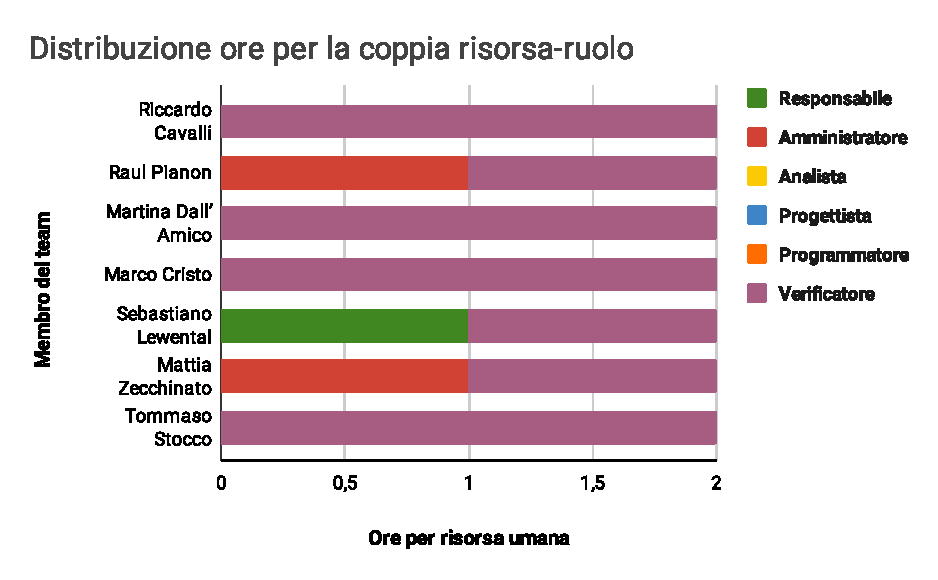
\includegraphics[width=0.90\textwidth]{assets/Preventivo/Sprint-14/distribuzione_ore_risorsa_ruolo.pdf}
  \caption{Sprint 14 - Istogramma della distribuzione oraria per la coppia risorsa-ruolo}
\end{figure}

\begin{figure}[H]
  \centering
  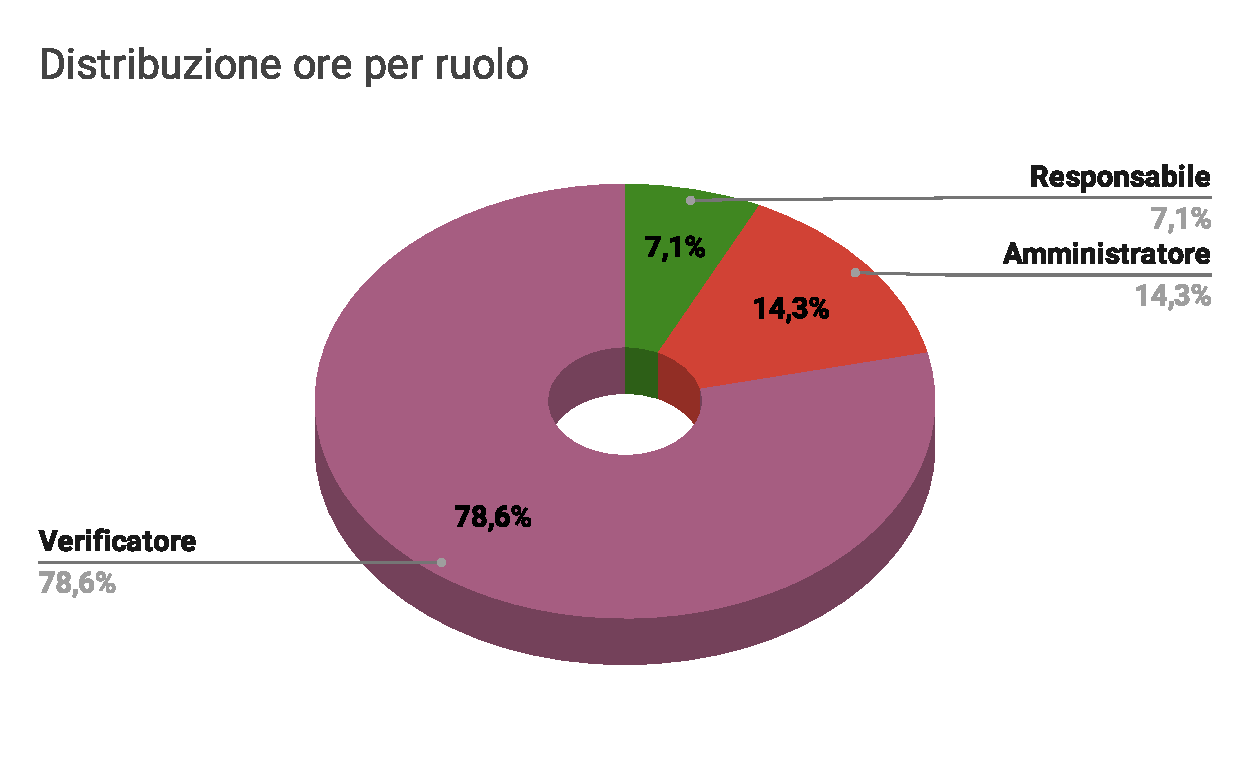
\includegraphics[width=0.90\textwidth]{assets/Preventivo/Sprint-14/distribuzione_ore_ruolo.pdf}
  \caption{Sprint 14 - Areogramma della distribuzione oraria per ruolo}
\end{figure}

\begin{minipage}{\textwidth}
Di seguito è riportato il preventivo economico del quattordicesimo \glossario{sprint}:
\begin{table}[H]
  \centering
  \begin{tabular}{|c|c|c|}
    \hline
    \multicolumn{3}{|c|}{\textbf{Preventivo economico}} \\
    \hline
    \textbf{Ruolo} & \textbf{Ore per ruolo} & \textbf{Costo (in \texteuro)} \\
    \hline
    \Responsabile[U]{} & 1 & 30,00 \\
    \hline
    \Amministratore[U]{} & 2 & 40,00 \\
    \hline
    \Analista[U]{} & 0 & 0,00 \\
    \hline
    \Progettista[U]{} & 0 & 0,00 \\
    \hline
    \Programmatore[U]{} & 0 & 0,00 \\
    \hline
    \Verificatore[U]{} & 11 & 165,00 \\
    \hline
    \textbf{Totale} & 14 & \textbf{235,00} \\
    \hline
  \end{tabular}
  \caption{Sprint 14 - Preventivo economico}
\end{table}
\end{minipage}
